\documentclass[oneside, openany]{book}
\usepackage{cite}
\usepackage[italian]{babel}
\usepackage[utf8x]{inputenc}
\usepackage{graphicx}
\usepackage{subfig}
\usepackage{amsfonts}
\graphicspath{{./images/}}
\usepackage{mathtools}
\usepackage{amsmath}
\usepackage{cases}
\usepackage{braket}
\usepackage{pdfpages}
\usepackage{multirow}
\usepackage{parskip}
\title{Riassunto dell'elaborato}
\date{3-10-2020}
\author{Alessia Lombarda}

\begin{document}
	\begin{titlepage}
		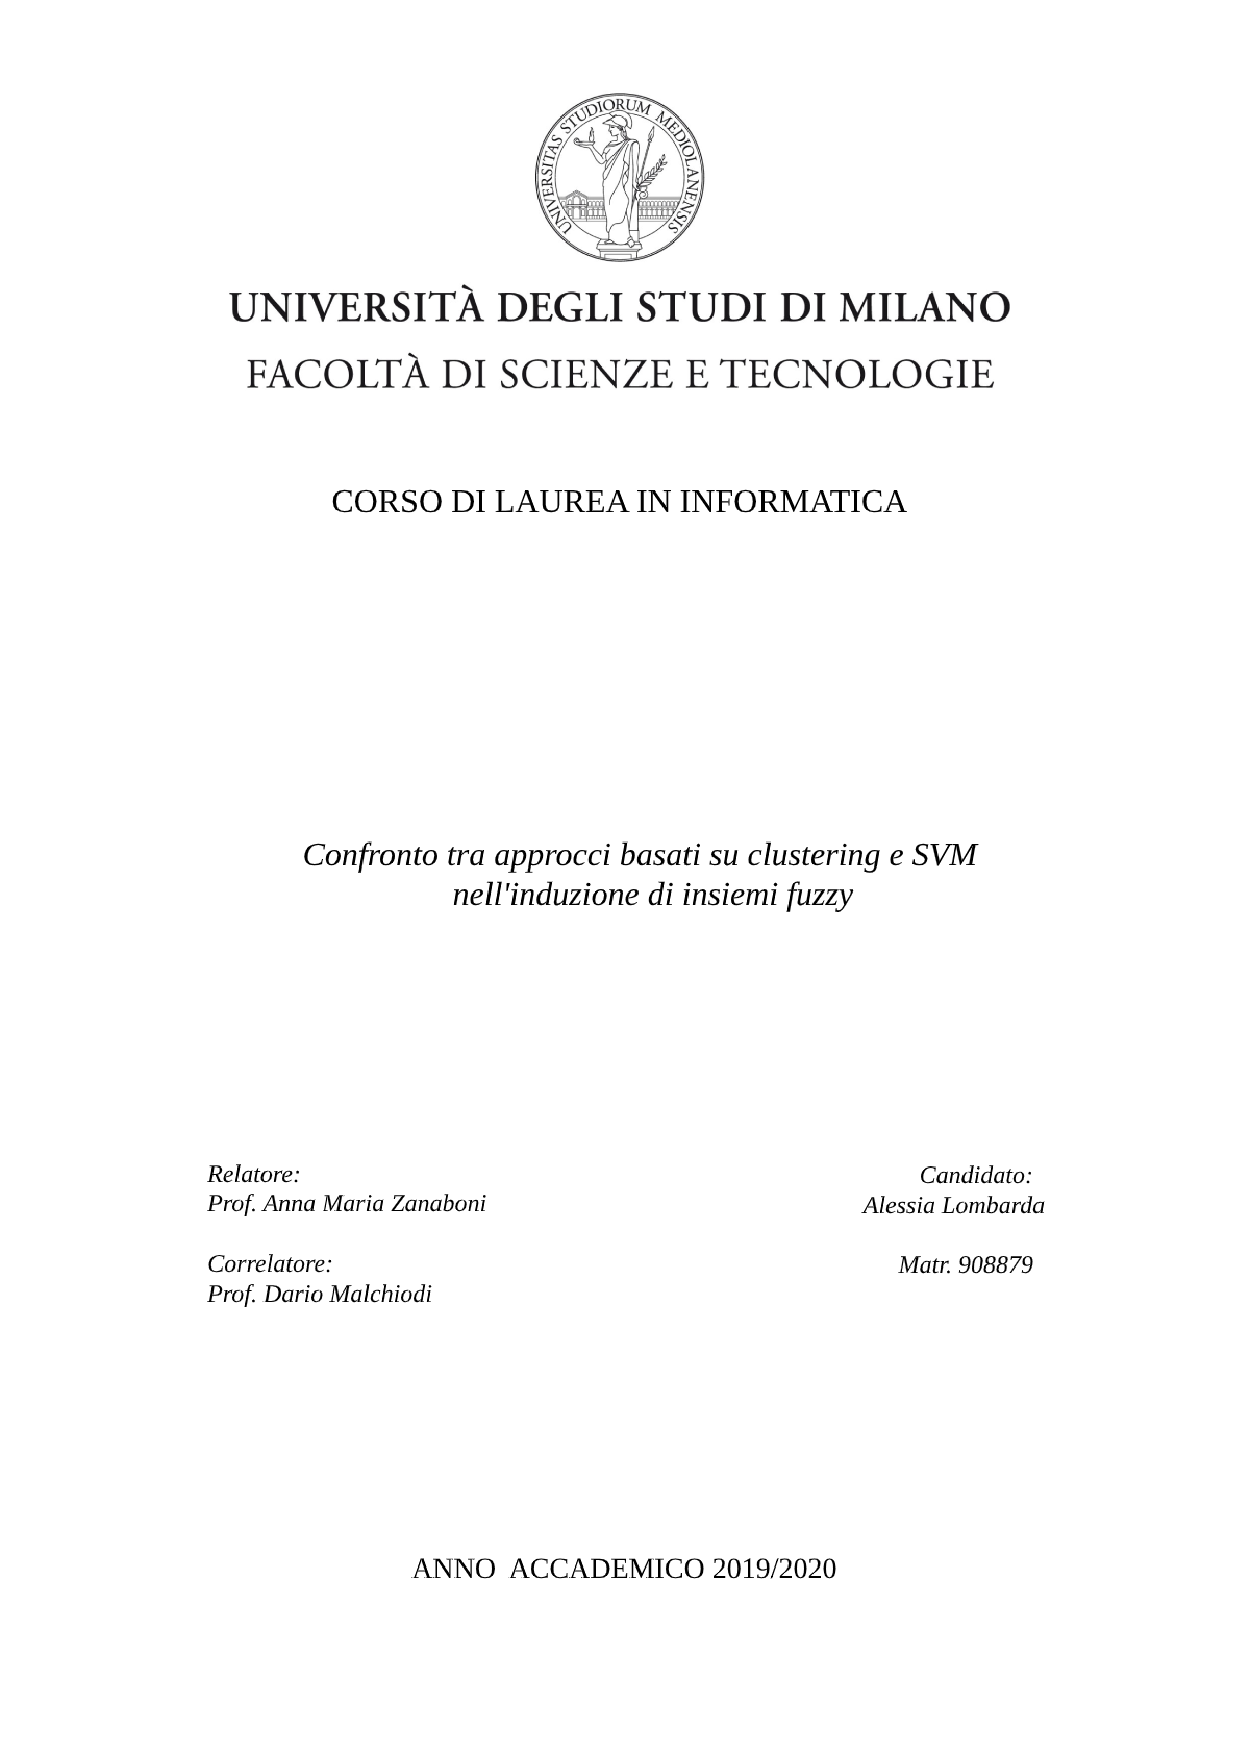
\includepdf{images/FRONTESPIZIO.pdf}
	\end{titlepage}
	\chapter*{Riassunto dell'elaborato}
	Questo elaborato descrive il lavoro di tirocinio che ho svolto presso l'Università degli Studi di Milano, in cui mi sono occupata della ricerca, modifica e confronto di implementazioni di algoritmi per l'induzione di funzioni di membership a insiemi fuzzy. La logica fuzzy e la teoria fuzzy sono vastamente diffuse nel campo dell'apprendimento automatico (e in particolare di quello supervisionato) in quanto modellano l'incertezza propria di gran parte realtà che ci circonda. Mentre nella logica classica un elemento può appartenere oppure no a un dato insieme, gli insiemi fuzzy sono descritti da una funzione di membership che determina il grado di appartenenza di un oggetto all'insieme in questione.\\
	Il problema dell'induzione della funzione di membership a un insieme fuzzy è complesso, anche a causa della mancanza di accordo sull'interpretazione della funzione stessa; il problema può essere approcciato in diversi modi: si sono approfonditi in questo elaborato i metodi riguardanti Fuzzy Clustering e Fuzzy Support Vector Machine.\\
	Tra i diversi algoritmi individuati sono stati scelti il Fuzzy C-Means (algoritmo di clustering) e la Fuzzy Support Vector Machine for Class Imbalance Learning. A partire dal codice reperito in rete lo si è modificato al fine di garantirne un funzionamento corretto e di migliorarne la leggibilità e le prestazioni. Si è infine svolta una valutazione sulle prestazioni degli algoritmi considerati, sui dataset Iris e Breast Cancer. Si è notato che l'algoritmo FCM ottiene prestazioni molto buone quando si lavora sulla membership alla classe setosa, che è linearmente separabile dalle altre, mentre ottiene prestazioni discrete sulla definizione della membership alle altre due classi, così come sul dataset Breast Cancer. L'algoritmo FSVM-CIL ottiene invece prestazioni discrete su entrambi i dataset, ma il suo funzionamento è oneroso in termini di tempo.
	
	L'elaborato è strutturato come segue: nel Capitolo 1 si descrivono le basi dell'apprendimento automatico (nello specifico di quello supervisionato); successivamente viene spiegato il funzionamento generale di un algoritmo di apprendimento, vengono definite le metriche che saranno poi utilizzate negli esperimenti e le tecniche di cross-validation e model selection. Viene inoltre introdotta la logica fuzzy e la sua estensione agli insiemi, e si inizia a delineare il problema dell'induzione della funzione di memberhship. Nel Capitolo 2 si introducono le macroclassi di algoritmi per l'induzione della funzione di membership: dopo una panoramica sul funzionamento generale degli algoritmi di clustering e support vector machine e dei corrispettivi fuzzy, si analizzano nel dettaglio il metodo FCM e l'algoritmo FSVM-CIL. Nel Capitolo 3, infine, si mostrano i dataset utilizzati negli esperimenti effettuati, le problematiche riscontrate nel codice reperito e le soluzioni individuate. Successivamente si illustrano i risultati ottenuti, che vengono poi analizzati anche grazie all'uso di rappresentazioni grafiche.
\end{document}